\begin{figure}
\centering	
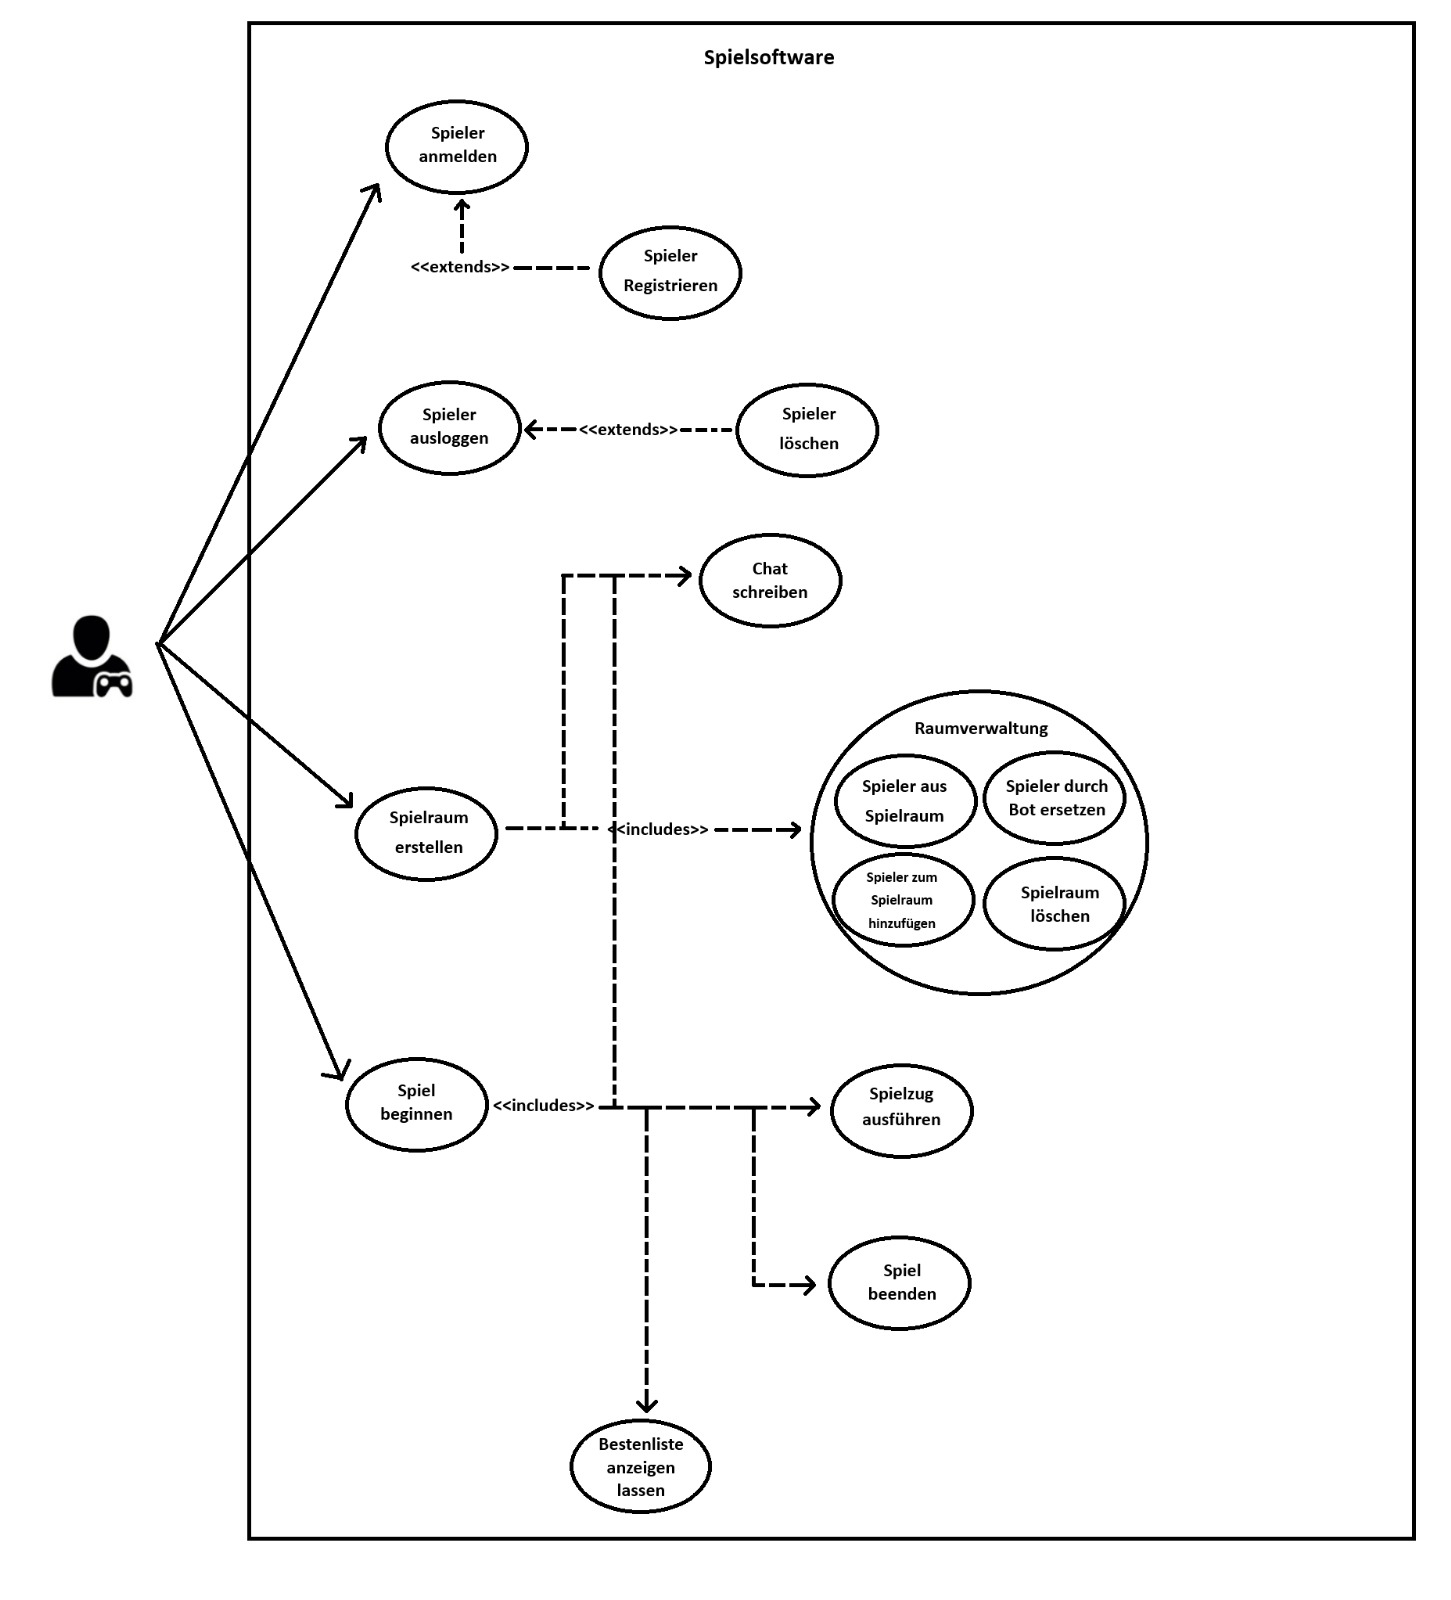
\includegraphics[width=0.9\textwidth]{SEP_Lasten_Pflichtenheft/img/systemedge.jpg}
\label{fig:sys}
\caption{Das Systemgrenzendiagramm}
\end{figure}

\section{Systemgrenze (Use Case Diagramm)}

Die Systemgrenze wird in der Abbildung~\ref{fig:sys} dargestellt


\section{Beschreibungen der Anwendungsfälle}

\newcounter{uc}\setcounter{uc}{10}

\begin{description}[leftmargin=5em, style=sameline]

	\begin{lhp}{uc}{UC}{uc:registrieren}
		\item [Name:] Spieler registrieren.
		\item [Ziel:] Spieler registriert sich im Spiel.
		\item [Akteure:] Spieler.
		\item [Vorbedingungen:] Spieler hat noch keinen Account und befindet sich auf der Login/Registrierungs Seite.
		\item [Eingabedaten:] Zugriffsdaten~\ref{daten:benutzername}Passwort~\ref{daten:passwort}.
		\item [Beschreibung:] Spieler registriert sein Konto.
		\item [Ausnahmen:] Der Benutzername ist bereits vergeben. Das System sendet eine Fehlermeldung.
		\item [Ergebnisse und Outputdaten:] Ein neues Konto wird erstellt. Der Spieler wird angemeldet und in die Lobby versetzt. 
		\item [Systemfunktionen] \ref{funk:zugriff}.
	\end{lhp}
	
	\begin{lhp}{uc}{UC}{uc:anmeld}
		\item [Name:] Spieler anmelden.
		\item [Ziel:] Spieler meldet sich im System an.
		\item [Akteure:] Spieler.
		\item [Vorbedingungen] Spieler ist auf der Registrierungsseite.
		\item [Eingabedaten:] Zugriffsdaten~\ref{daten:benutzername}Passwort~\ref{daten:passwort}.
		\item [Beschreibung:] Spieler meldet sich an.							
		\item [Ausnahmen:] \hfill
			\begin{itemize} 
				\item[] \textit{Passwort oder Benutzername ist falsch:} Das System zeigt eine Fehlermeldung an und der Spieler ist dazu aufgefordert eine erneute Anmeldung zu vollziehen.
				
			\end{itemize}
		\item [Ergebnisse und Outputdaten:] Spieler ist in der Lobby und sieht die Lobby-Seite.
		\item [Systemfunktionen:] \ref{funk:zugriff}.
	\end{lhp}
	
	\begin{lhp}{uc}{UC}{uc:löschen}
		\item [Name:] Spieler löschen.
		\item [Ziel:] Spieler entfernt seine Daten aus dem System.
		\item [Akteure:] Spieler.
		\item [Vorbedingungen] Spieler ist auf der Lobby-Seite.
		\item [Eingabedaten:] Zugriffsdaten~\ref{daten:benutzername}~\ref{daten:passwort}.
		\item [Beschreibung:] Spieler löscht das eigene Konto komplett.
		\item [Ausnahmen:] \hfill
			\begin{itemize} 
				\item[] \textit{Zugriffsdaten sind falsch:} Das System zeigt eine Fehlermeldung an, der Spieler bleibt auf der Seite und kann die Daten erneut eingeben.
			\end{itemize}
		\item [Ergebnisse und Outputdaten:] Spieler wird zur Login-Seite überführt, Spielerkonto wurde gelöscht.	
		\item [Systemfunktionen:] \ref{funk:zugriff}.
	\end{lhp}
    
    \begin{lhp}{uc}{UC}{uc:spielbeginnen}
    \item [Name:] Spiel beginnen.
    \item [Ziel:] Das System startet das Spiel
    \item [Akteure:] System, Spieler
    \item [Vorbedingungen:] Die erforderliche Anzahl an Spielern befindet sich im Spielraum und hat die Ready Checkbox ausgefüllt.
    \item [Eingabedaten:] Benutzername~\ref{daten:benutzername}.
    \item [Beschreibung:] Das Spiel wird gestartet, die Spieler werden zu der Spielbrett-Seite überführt. Das System initialisiert die Spiellogik.
    \item [Ausnahmen:] \hfill
        \begin{itemize}
            \item[] \textit{D:Alle Spieler sind bereit, aber das System startet das Spiel nicht} Das System zeigt eine Fehlermeldung und versucht das Spiel erneut zu starten.
        \end{itemize}
    \item [Ergebnisse und Outputdaten:] Das Spiel beginnt, die Spieler sind auf der Spielbrett-Seite
    \item [Systemfunktionen:] \ref{funk:spielverw}
    \end{lhp}

    \begin{lhp}{uc}{UC}{uc:spielbeenden}
    \item [Name:] Spiel beenden.
    \item [Ziel:] Das System beendet das Spiel, wertet das Ergebnis aus und aktualisiert ggf. Statistiken.
    \item [Akteure:] System
    \item [Vorbedingungen:] Ein Spiel ist derzeit aktiv und ein Spieler oder Bot hat 7 Gewinnpunkte
    \item [Eingabedaten:] Benutzername~\ref{daten:benutzername}, Gewinnpunkte im Spiel~\ref{daten:gw_punkte}, Siege~\ref{daten:siege}.
    \item [Beschreibung:] Das Spiel wird automatisch vom System beendet. Die Ergebnisse werden ausgewertet und gespeichert.
    \item [Ausnahmen:] \hfill
        \begin{itemize}
            \item[] \textit{Kein laufendes Spiel:} Das System zeigt eine Fehlermeldung und versucht zu recovern.
        \end{itemize}
    \item [Ergebnisse und Outputdaten:] Das Spiel ist beendet; Ergebnisse werden gespeichert und ggf. die Bestenliste aktualisiert. Spieler werden in den Spielraum überführt.
    \item [Systemfunktionen:] \ref{funk:spielverw} \ref{funk:bestenliste}
    \end{lhp}

    \begin{lhp}{uc}{UC}{uc:spielerausloggen}
    \item [Name:] Spieler ausloggen.
    \item [Ziel:] Der Spieler meldet sich vom System ab und beendet seine Sitzung.
    \item [Akteure:] Spieler.
    \item [Vorbedingungen:] Der Spieler ist eingeloggt.
    \item [Eingabedaten:] Benutzername~\ref{daten:benutzername}
    \item [Beschreibung:] Der Spieler wählt die Option zur Abmeldung. Das System beendet die Sitzung und schickt den Spieler zum Login-Screen zurück.
    \item [Ausnahmen:] \hfill
        \begin{itemize}
            \item[] \textit{Spieler wurde nicht ausgeloggt:} Das System zeigt eine Fehlermeldung an.
        \end{itemize}
    \item [Ergebnisse und Outputdaten:] Der Spieler ist abgemeldet und der Nutzer befindet sich im Login-Screen.
    \item [Systemfunktionen:] \ref{funk:zugriff}
    \end{lhp}

    \begin{lhp}{uc}{UC}{uc:spielzugausfuehren}
    \item [Name:] Spielzug ausführen.
    \item [Ziel:] Der Spieler führt während seines Spielzugs eine gültige Aktion gemäß den Regeln von Cosmic Eidex aus.
    \item [Akteure:] Spieler, System.
    \item [Vorbedingungen:] Das Spiel läuft (es wurde gestartet und die 36 Karten wurden verteilt) und der Spieler ist am Zug. Die Trumpffarbe steht fest und die vorherigen Stiche wurden abgeschlossen, weiterhin wurden alle Cosmic-Charakter-Effekte verarbeitet.
    \item [Eingabedaten:] Benutzername~\ref{daten:benutzername}, Spielzustand~\ref{daten:gamestate}.
    \item[Beschreibung:]
        \begin{enumerate}
             \item Da der Spieler an der Reihe ist, wird er zur Auswahl einer Karte oder Charakteraktion aufgefordert.
              \item Der Spieler wählt eine Karte aus oder aktiviert einen Charaktereffekt.
              \item Die Gültigkeit des Zuges wird geprüft:
              \begin{enumerate}
                    \item Bedienpflicht oder legaler Trumpf erlaubt.
                    \item Es darf nicht untertrumpft werden, wenn bereits ein Trumpf im Stich liegt.
                   \item Es werden die Cosmic-Charakter-Regeln beachtet.
              \end{enumerate}
              \item Wenn der Zug ungültig ist, wird eine Fehlermeldung gezeigt und Schritt 2 erneut ausgeführt.
              \item Ansonsten wird die Karte zum aktuellen Stich hinzu.
              \item Das System protokolliert den Spielzug
              \item Der folgende Spielverlauf wird geprüft:
                \begin{enumerate}
                    \item Mitspieler müssen noch spielen: Zugrecht wird an nächsten Spieler übergeben und Schritt 1 wird wieder ausgeführt.
                    \item Mitspieler müssen nicht mehr spielen: Stich wird beendet und Stichauswertung wird eingeleitet. ~\ref{uc:stichauswertung}
                \end{enumerate}
        \end{enumerate} 
    \item [Ausnahmen:] \hfill
        \begin{itemize}
            \item[] \textit{Ungültiger Spielzug:} Das System zeigt eine Fehlermeldung und akzeptiert den Zug nicht.
            \item[] \textit{Nicht der Zug des Spielers:} Das System blockiert die Aktion.
            \item[] \textit{Sphinx Effekt:} Karte wird zunächst verdeckt gelegt und erst später aufgedeckt.
            \item[] \textit{Charakterunterbrechung:} Es wird ein spezieller Flow eingeleitet und anschließend bei Schritt 6 weitergemacht.
        \end{itemize}
    \item [Ergebnisse und Outputdaten:] Der Spielzustand wurde entsprechend dem Spielzug aktualisiert. Spielzustand~\ref{daten:gamestate}
    \newline Dies beinhaltet:
    \begin{enumerate}
        \item Aktualisierung der Hand des Spielers
        \item Der Stich erhält eine neue Karte und Auspiel-Metadaten
        \item Das Zugrecht wechselt an den nächsten Spieler oder die Stichauswertung wird eingeleitet
        \item Es werden eventuell ausgelöste Charakter-Events protokolliert
    \end{enumerate}
    \item [Systemfunktionen:] \ref{funk:spielverw} \ref{funk:regelprüf} \ref{funk:stichverw} \ref{funk:chareffdipatch}
    \end{lhp}

    \begin{lhp}{uc}{UC}{uc:chatnachricht}
    \item [Name:] Chat schreiben.
    \item [Ziel:] Der Spieler sendet eine Nachricht im Spielraum-Chat oder Global-Chat.
    \item [Akteure:] Spieler.
    \item [Vorbedingungen:] Der Spieler befindet sich im Spielraum oder in der Lobby oder in der Spielbrett-Seite.
    \item [Eingabedaten:] Benutzername~\ref{daten:benutzername}, Chatnachricht~\ref{daten:msg}
    \item [Beschreibung:] Der Spieler gibt eine Nachricht ein und sendet sie. Das System zeigt sie allen Teilnehmern im Spielraum oder in der Lobby an.
    \item [Ausnahmen:] \hfill
        \begin{itemize}
            \item[] \textit{Leere oder ungültige Nachricht:} Das System versendet die Nachricht nicht.
        \end{itemize}
    \item [Ergebnisse und Outputdaten:] Die Chatnachricht wird allen Spielern im Spielraum oder der Lobby angezeigt.
    \item [Systemfunktionen:] \ref{funk:chat} 
    \end{lhp}

    \begin{lhp}{uc}{UC}{uc:lobbyerstellen}
    \item [Name:] Spielraum erstellen.
    \item [Ziel:] Der Spieler erstellt einen neuen Spielraum, um ein Spiel zu hosten.
    \item [Akteure:] Spieler, System.
    \item [Vorbedingungen:] Der Spieler ist eingeloggt und befindet sich in keinem Spielraum.
    \item [Eingabedaten:] Benutzername~\ref{daten:benutzername}, Spielraumname~\ref{daten:gameroom_name} optional Spielraumpasswort~\ref{daten:gameroom_password}
    \item [Beschreibung:] Der Spieler wählt die Option zum Erstellen einer neuen Lobby. Das System erstellt einen Spielraum und setzt den Spieler als Besitzer ein.
    \item [Ausnahmen:] \hfill
        \begin{itemize}
            \item[] \textit{Name bereits vergeben oder ungültig:} Das System zeigt eine Fehlermeldung und erstellt die Lobby nicht.
        \end{itemize}
    \item [Ergebnisse und Outputdaten:] Ein neuer Spielraum wird erstellt und der Spieler wird als Besitzer eingetragen.
    \item [Systemfunktionen:] \ref{funk:spielraum}
    \end{lhp}
    
    \begin{lhp}{uc}{UC}{uc:lobbyloeschen}
    \item [Name:] Spielraum löschen
    \item [Ziel:] Das System löscht einen Spielraum.
    \item [Akteure:] System
    \item [Vorbedingungen:] Der Spielraum ist leer.
    \item [Eingabedaten:] Spielraumname~\ref{daten:gameroom_name} Spielraumfüllung~\ref{daten:gameroom_pop}.
    \item [Beschreibung:] Das System löscht den Spielraum sobald sich kein Spieler mehr im Raum befindet
    \item [Ausnahmen:] \hfill
        \begin{itemize}
            \item[] \textit{Trotz Spielern wird ein Raum gelöscht:} Das System zeigt eine Fehlermeldung an.
        \end{itemize}
    \item [Ergebnisse und Outputdaten:] Der Spielraum wird gelöscht.
    \item [Systemfunktionen:] \ref{funk:spielraum}
    \end{lhp}
    
    \begin{lhp}{uc}{UC}{uc:spielerlobbyhinzufuegen}
    \item [Name:] Spielraum beitreten
    \item [Ziel:] Ein Spieler tritt einem bestehenden Spielraum bei, um am Spiel teilzunehmen.
    \item [Akteure:] Spieler, System.
    \item [Vorbedingungen:] Der Spielraum existiert und hat einen freien Platz.
    \item [Eingabedaten:] Benutzername~\ref{daten:benutzername}, Spielraumname~\ref{daten:gameroom_name}, Spielraumfüllung~\ref{daten:gameroom_pop} optional Spielraumpasswort~\ref{daten:gameroom_password}.
    \item [Beschreibung:] Der Spieler wählt einen Spielraum aus. Das System fügt den Spieler hinzu, wenn die Bedingungen erfüllt sind.
    \item [Ausnahmen:] \hfill
        \begin{itemize}
            \item[] \textit{Raum ist voll:} Das System zeigt eine Fehlermeldung und lässt keinen Beitritt zu.
            \item[] \textit{Raum nicht gefunden:} Das System zeigt eine Fehlermeldung an.
            \item[] \textit{Falsches Passwort:} Das System zeigt eine Fehlermeldung an.
        \end{itemize}
    \item [Ergebnisse und Outputdaten:] Der Spieler ist dem Spielraum beigetreten und sieht die anderen Teilnehmer.
    \item [Systemfunktionen:] \ref{funk:spielraum}
    \end{lhp}

    \begin{lhp}{uc}{UC}{uc:spielerauslobbyentfernen}
    \item [Name:] Spieler aus Spielraum entfernen.
    \item [Ziel:] Der Besitzer entfernt einen Spieler aus dem aktuellen Spielraum.
    \item [Akteure:] Lobbybesitzer.
    \item [Vorbedingungen:] Der Spielraum existiert und der ausführende Benutzer ist der Besitzer.
    \item [Eingabedaten:] Benutzername~\ref{daten:benutzername}
    \item [Beschreibung:] Der Besitzer wählt einen Spieler aus, der entfernt werden soll. Das System entfernt diesen Spieler aus dem Spielraum.
    \item [Ausnahmen:] \hfill
        \begin{itemize}
            \item[] \textit{Benutzer ist nicht der Besitzer:} Das System verweigert die Aktion.
            \item[] \textit{Spieler konnte nicht entfernt werden:} Das System zeigt eine Fehlermeldung an.
        \end{itemize}
    \item [Ergebnisse und Outputdaten:] Der ausgewählte Spieler wird aus dem Spielraum entfernt und in die Lobby zurückversetzt.
    \item [Systemfunktionen:] \ref{funk:spielraum}
    \end{lhp}

    \begin{lhp}{uc}{UC}{uc:botersetzen}
    \item [Name:] Spieler durch Bot ersetzen.
    \item [Ziel:] Eine freie Stelle im Spielraum wird mit einem Bot aufgefüllt.
    \item [Akteure:] Spielraum-Besitzer, System
    \item [Vorbedingungen:] Es gibt eine freie Stelle im Spielraum oder das Spiel läuft schon und ein Spieler verlässt die Sitzung
    \item [Eingabedaten:] Keine.
    \item [Beschreibung:] Der Besitzer wählt die Option aus einen Bot zum Spielraum hinzuzufügen, das System fügt den Bot hinzu. Falls ein Spieler im Spiel den Gameroom verlässt wird automatisch ein bot hinzugefügt, der das Spiel für den Spieler weiterspielt.
    \item [Ausnahmen:] \hfill
        \begin{itemize}
            \item[] \textit{Keine freie Stelle vorhanden:} Die Option zum auswählen ist nicht anklickbar.
        \end{itemize}
    \item [Ergebnisse und Outputdaten:] Eine Stelle im Spielraum ist nun mit einem Bot besetzt.
    \item [Systemfunktionen:] \ref{funk:spielverw}, \ref{funk:bots}.
    \end{lhp}

    \begin{lhp}{uc}{UC}{uc:bestenlisteanzeigen}
    \item [Name:] Bestenliste anzeigen lassen.
    \item [Ziel:] Der Spieler sieht die Bestenliste mit der Anzahl der gewonnenen Spiele aller Spieler.
    \item [Akteure:] Spieler.
    \item [Vorbedingungen:] Der Spieler befindet sich im Spielraum oder Vorraum.
    \item [Eingabedaten:]
    \item [Beschreibung:] Das System zeigt eine Bestenliste auf Basis der Spielstatistiken an, dies tut es als Teil der GUI.
    \item [Ausnahmen:] \hfill
        \begin{itemize}
            \item[] \textit{Bestenliste nicht verfügbar:} Das System zeigt eine Fehlermeldung anstelle der Bestenliste an
        \end{itemize}
    \item [Ergebnisse und Outputdaten:] Die Bestenliste mit der Anzahl gewonnener Spiele wird angezeigt.
    \item [Systemfunktionen:] \ref{funk:bestenliste}
    \end{lhp}

    \begin{lhp}{uc}{UC}{uc:stichauswertung}
    \item [Name:] Stichauswertung
    \item [Ziel:] Der Stich wird anhand der Spielregeln ausgewertet.
    \item [Akteure:] System
    \item [Vorbedingungen:] Alle Spieler waren am Zug und der Stich muss ausgewertet werden.
    \item [Eingabedaten:] Trumpffarbe ~\ref{daten:trumpf} aktueller Stick ~\ref{daten:stich} 
    \item [Beschreibung:] Das System schaut sich die Stichkarten an und verteilt den Stich an den gewinnenden Spieler.
    \item [Ausnahmen:] \hfill
        \begin{itemize}
            \item[] \textit{System kann auf benötigte Daten nicht zugreifen:} Das System zeigt eine Fehlermeldung an.
        \end{itemize}
    \item [Ergebnisse und Outputdaten:] Der Stich wurde an den gewinnenden Spieler vergeben, und eine neue Spiel/Kartenlegrunde wird initialisiert
    \item [Systemfunktionen:] \ref{funk:bestenliste}
    \end{lhp}
\end{description}